\documentclass{article}
\setcounter{tocdepth}{2}

\usepackage{tikz}
\usepackage{amsthm}
\usepackage{amsmath}
\usepackage{amsfonts}
\usepackage{graphicx,paralist}
\usepackage[titlenumbered,ruled]{algorithm2e}
\usepackage{float}
 
\theoremstyle{definition}
\newtheorem{definition}{Definition}[section]

\theoremstyle{lemma}
\newtheorem{lemma}{Lemma}[section]

\theoremstyle{corollary}
\newtheorem{corollary}{Corollary}[section]

\theoremstyle{theorem}
\newtheorem{theorem}{Theorem}[section]

\begin{document}

\begin{titlepage}

\begin{center}
\includegraphics[scale=0.4]{Logo-UNIPisa.jpg} 
\end{center}

\begin{center}
    {\LARGE{\bf An FPT algorithm for approximated treewidth}}\\
    \vspace{5mm}
    {\large{\bf Algorithm Design - final exam}}\\
    \vspace{2.5mm}
	{\large{\bf Laura Bussi}}\\
\end{center}
\end{titlepage}

\newpage

\tableofcontents

\newpage

\section{Introduction}
In this report we present the notion of \emph{Fixed Parameterized Tractability} as a tool to improve the tractability of known NP problems. First of all, parameterized complexity is introduced and intuitively explained. In section 2, we consider treewidth computation as an NP-complete problem which admits an FPT (approximated) algorithm and introduce Vertex Coloring as a case study. In section 3, we focus on the Bodlaender's algorithm for approximated treewidth and its analysis. In section 4 we further investigate the application of treewidth to the Vertex Coloring problem, toghether with other examples.

\subsection{Parameterized complexity}
Many real life problems are optimization ones. Let us think about the registers
allocation task for a compiler, or the job scheduling problem: all of these are known
to be NP-complete and usually require exponential time to be solved. \\
Of course, we cannot simply ignore them, then we have to deal with their complexity and try to obtain some kind of feasibility, in order to get a solution. \\
A well known approach is by using \emph{approximation}: instead of searching for an optimal solution, we compute an approximate one. This usually allows for a more convenient computational time. However, in many cases, we can compute a fast and exact solution for certain instances of a problem by exploiting its structure, which gives us some useful "extra" information. \\
Parameterized complexity was first introduced by Downey and Fellows in 1999~\cite{downey}. The main idea is to fix some part of the input as a parameter, such that we can confine the combinatorial explosion to a function of it. In this way, we can build an algorithm which is polynomial in the size of the input and which can lead to the exact result or to an approximation. This kind of approach falls into the range of fine grained complexity, which tries to analize a problem with respect to its structure, in order to get a more precise idea of its computational complexity, under the assumption that P $\not =$ NP holds. \\
Roughly speaking, we can summarize as follows:
\begin{itemize}
	\item In classical complexity theory, the cost of an algorithm is expressed as a 
	function of the input size;
	\item In parameterized complexity, we exploit the structure of the problem in some way to
	fix a parameter and express the cost of the solving algorithm as a function of it.
\end{itemize}
Parameterized complexity carries several advantages in algorithm design, due to the fact that it is possible to achieve a certain tractability for a problem: in general, we search for a $f(k)n^
c$ running time. Note that this could be exponential w.r.t. the parameter $k$, but it is polynomial w.r.t. the input size. Then FPT algorithms are known to work well with "small" parameters. \\
In the following, we focus on a class of parameterized problems and see how to solve them exploiting this notions.

\section{Parameterized problems}
Let us start by remarking that there exist many problems which we are not known to be FPT, as for instance \emph{k-clique} and \emph{Dominating Set}~\cite{kclique}. However, proving this requires some strong assumptions besides P$\not =$NP and its beyond the scope of this report.  \\
However, many interesting problems can be solved by using FPT-algorithms. In this report, we focus on the problem of computing the \emph{treewidth} of a graph. \\
Treewidth is important in several fields and can find an enormous number of applications, as for instance in CSP solving or in computing string edit distance, thus having an efficient algorithm for it plays a fundamental role for a wide class of problems. In the following we give some basic definitions and present the general problem. We'll then introduce the Vertex Coloring problem as an example of an application of treewidth.

\subsection{Tree decomposition and treewidth}
The definition of treewidth rises naturally from the concept of \emph{tree decomposition} of a graph. Tree decomposition allows us to check if a graph is \emph{tree like}: intuitively, this holds if its treewidth is "small" enough. A tree has treewidth 1.
\theoremstyle{definition}
\begin{definition}
	A tree decomposition for a graph $G = (V, E)$ consists of a tree $T$ and a set
	$X = \{ X_t \mid X_t \subseteq V, t \in T \}$ (called \emph{bags}) such that:
	\begin{itemize}
		\item for each node $g \in V$ there exists $t \in T$ such that $g \in X_t$.
		\item for each edge $(g,h) \in E$ there exists $t \in T$ such that $g \in X_t$
		and $h \in X_t$.
		\item given $t_1, t_2, t_3 \in T$ such that $t_2$ lies on a path from $t_1$ to
		$t_3$, if a node $v \in V$ belongs to $X_{t_1}$ and $X_{t_3}$, then it belongs also
		to $X_{t_2}$.
	\end{itemize}
\end{definition}
We can now define the treewidth of a graph.
\theoremstyle{definition}
\begin{definition}
	The width of a tree decomposition $(T, X)$ is
	\begin{center}
		$width((T,X)) = max_t \mid X_t \mid -1$.
	\end{center}
	The treewidth of a graph $G$ is the minimum width of any of its tree decomposition.
\end{definition}

In Figure~\ref{tdec} an example of graph with one of its tree decompositions.

\begin{figure}[H]
	\begin{center}
		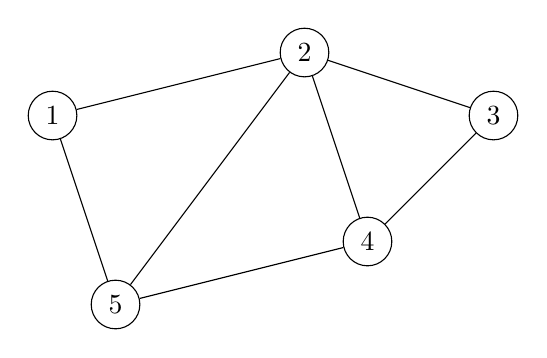
\begin{tikzpicture}
  			[scale=.8,auto=left,every node/.style={circle, draw,}]
  			\node (n4) at (4,8)  {1};
  			\node (n5) at (8,9)  {2};
  			\node (n1) at (11,8) {3};
  			\node (n2) at (9,6)  {4};
  			\node (n3) at (5,5)  {5};
		
  			\foreach \from/\to in {n5/n3,n4/n5,n5/n1,n1/n2,n2/n5,n2/n3,n3/n4}
    		\draw (\from) -- (\to);
		\end{tikzpicture}
		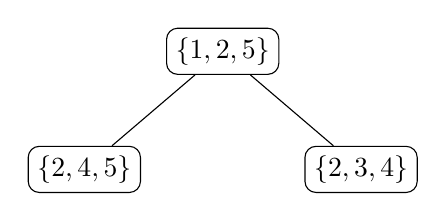
\begin{tikzpicture}[sibling distance=10em,
 			every node/.style = {shape= rectangle, rounded corners, draw, align=center,}]]
  			\node {$\{1,2,5\}$}
    		child { node {$\{2,4,5\}$} }
    		child { node {$\{2,3,4\}$}
			};
		\end{tikzpicture}
	\end{center}
	\caption{A small graph, with one of its tree decompositions. For each tree decomposition of 
	the graph, we have $max_t \mid X_t \mid \geq 3$, hence the graph has treewidth $2$.}
    \label{tdec}
\end{figure}

The problem to determine whether a graph has treewidth at most $k$ or not is NP-hard: the exahustive algorithm to compute it for a graph $G$ is exponential in the size of the input. The existence of an exact polynomial algorithm for treewidth is still an open problem, but we can compute a 5-approximation in $O(c^kn)$ time. \\
Let us now introduce another definition that will be useful later, when we'll face Vertex Coloring.
\theoremstyle{definition}
\begin{definition}
	A \emph{(standard) nice tree decomposition} is a tree decomposition $(X, T)$ where 
	$X = \{X_{t_1},...,X_{t_n}\}$, $T$ is a rooted tree and:
	\begin{itemize}
		\item every bag of $T$ has at most two children;
		\item if a bag $X_i$ has two children $X_j$ and $X_{j'}$, 
		then $X_i = X_j = X_j'$ (\emph{join node});
		\item if a bag $X_i$ has one children $X_j$, then either:
		\begin{itemize}
			\item $\mid X_i \mid = \mid X_j \mid + 1$ and $X_j \subset X_i$ 
			(\emph{introduce node})
			\item $\mid X_i \mid = \mid X_j \mid - 1$ and $X_i \subset X_j$ 
			(\emph{forget node})
		\end{itemize}
	\end{itemize}
	A bag of $T$ with no children is called a \emph{leaf}.
\end{definition}

\begin{lemma}
	Given a graph $G$ and a tree decomposition of $G$ of width $w$, we can compute a (standard)
	nice tree decomposition of $G$ of width $w$ and $O(wn)$ nodes in time $O(w^2n)$.
\end{lemma}

\subsection{A case study: Vertex Coloring}
Let us now introduce the problem of Vertex Coloring as a case study and let us see that not every choice of a parameter leads to FPT algorithms. Note that Vertex Coloring is easily solvable by using treewidth: more on this later on.
\theoremstyle{definition}
\begin{definition}
	A \emph{vertex coloring} is an assignment of labels or colors to each vertex of a graph
	such that no edge connects two identically colored vertices. \\
	A vertex coloring that minimize the number of colors needed for a given graph $G$ is 
	known as a \emph{minimum vertex coloring} of $G$.
\end{definition}
Now we might like to solve VC by fixing as a parameter $k$ the number of colors to be used. Let us see that this is not a suitable choice: we recall here that we work under the assumption of P 
$\not =$ NP.~\cite{palgo} \\
Since we have fixed $k$ as the number of colours, we would like to obtain an $f(k)n^c$-time algorithm for solving VC. But we know that deciding if a graph has a proper $k$-coloring is NP-complete, thus such an algorithm would imply P$=$NP. At the same manner, an XP algorithm having running time $f(k)n^{g(k)}$ would imply $P = NP$, hence Vertex Coloring is not FPT with respect to the number of colors.

\section{An FPT-algorithm for approximated treewidth}
Now we can introduce an algorithm for computing approximated treewidth in polynomial time (w.r.t to the input size $n$): this has been developed by Bodlaender et al. in 2013~\cite{approx}. In the following we'll focus on the 3-approximation $O(c^k nlogn)$ algorithm, giving its main procedures and data structures togheter with some intuitive explanations, without going in dept into details, since it would require many technicisms which could be difficult to appreciate. The $O(c^k n)$ 5-approximation algorithm is just an evolution from the former: also for this we'll give the main ideas used to reach the linear time goal, without filling them with many techincisms. We remind to the original paper for further readings. \\
The linear time algorithm computes a tree decomposition of a graph $G$ of width at most $5k+4$ or reports a failure if the width is more than $k$. This algorithm leads to a 5-approximation of the solution: faster algorithms, where faster means that they are not exponential w.r.t. the parameter $k$ have been developed, but they compute a $k^2$ approximation of the tree decomposition as e.g. in~\cite{k2algo}.

\subsection{Useful definitions and lemmas}
We first give some definitions and lemmas that will be necessary in order to understand the algorithm.
\theoremstyle{definition}
\begin{definition}
	Given a graph $G$ and an integer $k$, the \emph{improved} graph of $G$, denoted as $G_I$ is
	obtained by adding an edge between each pair of vertices with at least $k+1$ common
	neighbors of degree at most $k$ in $G$.
\end{definition}
A vertex $v$ of $G$ is said to be \emph{simplicial} if its neighborhood is a clique. It is said to be \emph{I-simplicial} if it is simplicial in the improved graph. Since the vertices connected by the added edges will be in the same bag during the construction of any tree decomposition, then no tree decomposition will be spoiled if we compute it on the improved graph. This is stated by the following lemma:
\begin{lemma}
	Given a graph $G$ and a positive integer $k$, $twidth(G) \leq k$ if and only if 
	$twidth(G_I) \leq k$ 
\end{lemma}
Intuitively, all the neighbors of an I-simplicial vertex must be contained in the same bag when computing the tree decomposition of $G$, thus we can safely remove the I-simplicial vertices from $G_I$, compute the tree decomposition and then reintroduce them. If no large set of I-simplicial vertices can be found, then we can identify a large matching. \\
The main ingredients of the algorithm are stated by the following lemma:
\begin{lemma}\label{lem}
	There is an $O(k^{O(1)}n)$ algorithm that, given a graph $G$ and an integer $k$, either
	\begin{itemize}
		\item returns a maximal matching in $G$ of cardinality at most $\mid V \mid /O(k^6)$
		\item returns a set of $\mid V \mid /O(k^6)$ I-simplicial vertices or
		\item correctly concludes that the treewidth of $G$ is larger than $k$
	\end{itemize}
	Furthermore, if a set $X$ of I-simplicial vertices is computed and the algorithm is provided
	with some tree decomposition $\mathcal{T_I}$ of $G_I \setminus X$ of width at most $k$, 
	then one can turn $\mathcal{T_I}$ into a tree decomposition $\mathcal{T}$ of $G$ of width at
	most $k$ (or conclude that the treewidth of $G$ is larger than $k$) in $O(k^{O(1)}n)$ time.
\end{lemma}
This allows to reduce the problem to a \emph{compression} variant, where we are given a graph
$G$, an integer $k$ and a tree decomposition of $G_I$ of width at most $k$ and we want to either conclude that the treewidth of $G$ is at least $k$ or output a tree decomposition of $G$ of width at most $3k+4$.

\subsection{The main procedure \textbf{Alg$_1$}}
We first provide the $O(c^knlogn)$ 3-approximation algorithm and then modify it in order to get a linear time 5-approximation algorithm. The former has several procedure: we first introduce the main procedure \textbf{Alg$_1$}.
According to Lemma~\ref{lem}, we have three cases.
\begin{itemize}
	\item If the application of the lemma concludes that $twidth(G) > 3k + 4$, then the algorithm stops.
	\item If a matching $M$ of size at least $n/O(k^6)$ is found, then we contract it to obtain $G'$:
	note that $twidth(G) \leq k \implies twidth(G') \leq k$. Then, \textbf{Alg$_1$} is applied 
	recursively to $G'$ in order to obtain a tree decomposition $\mathcal{T'}$ of it, having width 
	at most $3k + 4$.
	Thus, decontracting $M$ results in obtaining a tree decomposition $\mathcal{T}$ of $G$ of width 
	$6k + 9$: every vertex in the contracted graph is replaced by at most two vertices before the
	contraction. \\
	Finally, we apply the subprocedure \textbf{Compress$_1$} (see next section) to obtain a tree
	decomposition $\mathcal{T}$ of $G$ of width at most $3k + 4$ or to conclude that $twidth(G) > k$.
	\item If a large set $X$ of I-simplicial vertices is found, then we compute the improved graph $G_I$,
	remove $X$ from it, apply \textbf{Alg$_1$} recursively on $G_I \setminus X$ to get its tree
	decomposition $\mathcal{T'}$, again of width $3k + 4$ and finally try to reintroduce the vertices of
	$X$ in order to obtain a tree decomposition $T$ of $G$. If the reintroduction fails, then the
	algorithm concludes that $twidth(G) > k$ and stops; otherwise, since we want $S_0$ to be the root
	bag, we may have to run \textbf{Compress$_1$} again.
\end{itemize}

\begin{algorithm}[H]
	\SetAlgoLined
	\SetKwInOut{Input}{Input}
	\SetKwInOut{Output}{Output}
	\Input{A connected graph $G$, an integer $k$, and $S_0 \subseteq V$ s.t. 
	$\mid S_0 \mid \leq 2k+3$ and $G \setminus S_0$ is connected}
	\Output{A tree decomposition $\mathcal{T}$ of $G$ with $width(\mathcal{T} \leq 3k+4)$ 
	and $S_0$ as the root bag, or the conclusion that $twidth(G) > k$}
	\caption{The main procedure \textbf{Alg$_1$}}
	
	Run algorithm of Lemma~\ref{lem} for parameter $3k+4$;
	\If{conlusion that $twidth(G) > 3k+4$}{
		\KwRet $\bot$
	}
	\If{$G$ has a matching M of cardinality at least $n/O(k^6)$}{
		Contract $M$ to obtain $G'$;
		$\mathcal{T'} \leftarrow \textbf{Alg$_1$}(G',k)$ \\
		\eIf{$\mathcal{T'} = \bot$}{
			\KwRet $\bot$
		} {
		Decontract the edges of $M$ in $\mathcal{T'}$ to obtain $\mathcal{T}$ \\
		\KwRet $\textbf{Compress$_1$}(G,k,\mathcal{T})$
		}
	}
	\If{$G$ has a set $X$ of at least $n/O(k^6)$ I-simplicial vertices}{
		Compute the improved graph $G_I$ and remove $X$ from it \\
		$\mathcal{T'} \leftarrow \textbf{Alg$_1$}(G_I \setminus X,k)$ \\
		\If{$\mathcal{T'} = \bot$}{
			\KwRet $\bot$
		}
		Reintroduce vertices of $X$ to $\mathcal{T'}$ to obtain $\mathcal{T}$ \\
		\eIf{Reintroduction failed}{
			\KwRet $\bot$
		}{
			\KwRet $\textbf{Compress$_1$}(G,k,\mathcal{T})$
		}
	}
\end{algorithm}

\bigskip
All the given steps, excluding the recursive calls of \emph{Alg$_1$} and the subprocedure 
\emph{Compress$_1$} can be performed in $O(k^{O(1)}n)$ time. Providing that the running time of \textbf{Compress1} is $O(c^k nlogn)$ for some $c \in \mathbb{N}$, we obtain:
\[ T(n) \leq O(k^{O(1)}n) + O(c^k nlogn) + T((1 - 1/Ck^6) n)\]
By unravelling the recurrence we obtain the following result:
\[ T(n) \leq \sum_{i=0}^\infty (1 - 1/Ck^6)^i O(k^{O(1)}n + c^k nlogn) \]
\[ = Ck^6 O(k^{O(1)}n + c^k nlogn) = O({c_1}^k nlogn) \]
for some $c_1 > c$.

\subsection{The subprocedure \textbf{Compress$_1$}}
\begin{algorithm}[H]
	\SetAlgoLined
	\SetKwInOut{Input}{Input}
	\SetKwInOut{Output}{Output}
	\Input{A connected graph $G$, $k \in \mathbb{N}$, a set $S_0 \subseteq V$ s.t. 
	$\mid S_0 \mid \leq 2k+3$ and $G \setminus S_0$ is connected, and a tree decomposition
	$\mathcal{T}_{apx}$ with $twidth(\mathcal{T}_{apx} \leq O(k))$}
	\Output{A tree decomposition $\mathcal{T}$ of $G$ with $width(\mathcal{T} \leq 3k+4)$ 
	and $S_0$ as the root bag, or the conclusion that $twidth(G) > k$}
	\caption{The subprocedure \textbf{Compress$_1$}}
	
	Initialize data structre $\mathcal{DS}$ with $G,k,S_0,\mathcal{T}_{apx}$ \\
	\KwRet $\textbf{FindTD()}$
\end{algorithm}

\bigskip
The algorithm first initialise the data structure $\mathcal{DS}$, then run a recursive algorithm
\textbf{FindTD} that construct the decomposition, which is returned as a pointer to the root bag. The
initialisation of the data structre takes $O(c^k n)$ time, while the running time of \textbf{FindTD} is
$O(c^k nlogn)$.

\subsection{The data structure $\mathcal{DS}$}
Here we give a brief description of the data structure $\mathcal{DS}$, whose state is $G,k,\mathcal{T}$ and three subsets of vertices $S,X$ and $F$, besides a pin $\pi$ such that $\pi \not \in S$.
Intuitively, the meaning of these sets and the pin is as follows:
\begin{itemize}
	\item $S$ will serve as a root bag for some subtree
	\item $\pi$ indicates the current active component
	\item $U$ is the current active component, containing the vertex $\pi$
	\item $X$ is a balanced $S$-separator (of $G[S \cup U]$)
	\item $F$ is a set of vertices marking the connected components of $G[S \cup U] \setminus (S \cup X)$
	as "finished"
\end{itemize}
As said, the initialization of $\mathcal{DS}$ takes $O(c^k n)$ time. Each update and query takes
$O(c^k logn)$ time.

\subsection{The algorithm \textbf{FindTD}}
\begin{algorithm}[H]
	\SetAlgoLined
	\SetKwInOut{Data}{Data}
	\SetKwInOut{Output}{Output}
	\Data{Data structure $\mathcal{DS}$}
	\Output{Tree decomposition of width at most $3k + 4$ of $G[S \cup U]$ with $S$ as root bag
	or conclusion that $twidth(G) > k$}
	\caption{The algorithm \textbf{FindTD}}
	
	$old_S \leftarrow \mathcal{DS}.get_S()$ \\
	$old_\pi \leftarrow \mathcal{DS}.get_\pi()$ \\
	$sep \leftarrow \mathcal{DS}.findSSeparator()$ \\
	\If{ $sep = \bot$ } {
		\KwRet $\bot$
	}
	$\mathcal{DS}.insert_X(sep)$ \\
	$\mathcal{DS}.insert_X(\pi)$ \\
	$pins \leftarrow \emptyset$ \\
	\While{ $(u,l) \leftarrow \mathcal{DS}.findNextPin() \not = \bot$ } {
		$pins.append(u)$ \\
		$\mathcal{DS}.insert_F(u)$
	}
	$\mathcal{DS}.clear_X()$ \\
	$\mathcal{DS}.clear_F()$ \\
	$\mathcal{DS}.insert_S(sep)$ \\
	$bags \leftarrow \emptyset$ \\
	\For{ $u \in pins$ } {
		$\mathcal{DS}.set_\pi(u)$ \\
		$bags.append(\mathcal{DS}.findNeighborhood())$
	}
	$children \leftarrow \emptyset$ \\
	\For{ $u,b \in pins,bags$ } {
		$\mathcal{DS}.set_\pi(u)$ \\
		$\mathcal{DS}.clear_S()$ \\
		$\mathcal{DS}.insert_S(b)$ \\
		children.append(\textbf{FindTD()})
	}
	$\mathcal{DS}.clear_S()$ \\
	$\mathcal{DS}.insert_S(old_S)$ \\
	$\mathcal{DS}.set_\pi(old_\pi)$ \\
	\If{ $\bot \in children $ } {
		\KwRet $\bot$
	}
	\KwRet \textbf{build($old_S, sep, children$)}
\end{algorithm}

\bigskip
The algorithm first apply query findSSeparator ($k^O(1)$ running time), which either finds a 1/2-balanced $S$-separator in $G[S \cup U]$ of size at most $k+1$ or concludes that $twidth(G) >k$. If such a separator is found, then it is added to $X$ in the data structure. Since we add the pin $\pi$ to $sep$, and then also to $X$, we have $\mid sep \mid \leq k + 2$. \\
In the subsequent loop, query findNextPin ($O(1)$ running time) either finds a vertex $u$ of a connected component of $G[S \cup U] \setminus (S \cup X)$ that does not contain any vertex of $F$ or concludes that each of them contains at least one vertex of $F$. If $u$ is found, then we mark it by adding it to $F$ and proceed until all the components are marked. After this, the list $pins$ contains exactly one vertex for each connected component of $G[S \cup U] \setminus (S \cup sep)$. These vertices are then removed from $F$: hence $F$ become empty again. Note that the query findNextPin returns, as a the second component of the return value, also the size of the component containing $u$. Furthermore, the components are found in decreasing order w.r.t. size and this property plays a fundamental role in the linear time algorithm. \\
Since it will be no longer used, the set $X$ is made empty. On the other hand, $sep$ is added to $S$. The new $S$ will constitute the new bag, of size at most $\mid S \mid + \mid sep \mid \leq 3k + 5$. Now we have to compute the tree decomposition for the connected components below this bag, which are indicated by vertices listed in $pins$. \\
The components are processed one by one in the first for loop: for each vertex $u \in pins$, $u$ is set as the new pin. The set $U$ is redefined in such a way that it becomes the connected components containing considered $u$. Query findNeighborhood ($O(k)$ running time) finds the neighborhood of $U$ in $S$ or concludes that its cardinality is greater than $2k + 3$.

\subsection{Moving to the linear time 5-approximation}
The main idea to get a linear time algorithm starting from the one presented above is to first achieve a 
$O(c^k nlog^{(\alpha)}n)$ running time. This can be obtained with some modifications and improvements to the given procedures. In particular, the following are (re)defined:
\begin{itemize}
	\item \textbf{Alg$_\alpha$} behaves almost exactly as \textbf{Alg$_1$}, except for the call to the
	subprocedure \textbf{Compress$_1$}, which is replaced by \textbf{Compress$_\alpha$}.
	\item \textbf{Compress$_\alpha$} allows $S_0$ to be of size at most $4k + 3$ and returns a tree 
	decomposition of width at most $5k + 4$. As \textbf{Compress$_1$}, it initialises the data structure
	$\mathcal{DS}$ and calls the subprocedure \textbf{FindPartialTD}.
	\item \textbf{FindPartialTD} exploits the fact that connected components are returned in the
	descendent order of cardinalities. Then we continue to compute a partial tree decomposition only as
	long as the identified components are larger or equal to $logn$. The enumeration stops when we find
	a component having size smaller than $logn$: then all the remaining components are smaller than
	$logn$ and we can run the algorithm \textbf{Alg$_{\alpha - 1}$} on them.
\end{itemize}
To get the linear time algorithm, we consider only the case when $n$ is much larger than $k$: otherwise, the given algorithms have in fact already $O(c^k n)$ running time. Thus we focus on the cases in which we have:
\begin{itemize}
	\item $n$ much greater than $k$
	\item a tree decomposition $\mathcal{T}_{apx}$ of $G$, of width $O(k)$ at our disposal
\end{itemize}
In this case, we exploit the Bodlaender and Kloks dynamic programming algorithm~\cite{bodlaender}, which either computes a tree decomposition of $G$ of width at most $k$ or correctly concludes that $twidth(G)$ is larger than $k$. The running time of this algorithm is $O(2^{O(k^3)} n)$ and it can be turned into a tree automata based algorithm, having running time $O(2^{2×^{O(k^3)}} + n)$ if we inspect an entry of a table of size $O(2^{2^{O(k^3)}})$ in constant time. \\
Knowing this, it's easy to se that:
\begin{itemize}
	\item if $n \geq O(2^{2^{O(k^3)}})$, then the algorithm runs in $O(2n) = O(n)$, finding an optimal
	tree decomposition of $G$;
	\item otherwise, the $O(c^k nlog^{(3)}n)$ algorithm runs in time $O(c^k n)$ for the reasons mentioned
	above.
\end{itemize}
Hence the algorithm has running time $O(c^k n)$.

\section{Back to Vertex Coloring}
Let us now see how to parameterize Vertex Coloring via treewidth. We consider at first a 3-coloring problem for a given graph $G$.
\begin{lemma}
	Given a graph $G$ and a tree decomposition of $G$ of width $w$, 3-coloring can be solved in
	$O(3^wn)$ time.
\end{lemma}
We remark that $X_t$ is the set of vertices in the node $t$. Furthermore, we denote as $V_t$ the set of vertices appearing in the subtree rooted in $t$. Then, for every node $t$ and coloring $c: X_t \rightarrow \{1,2,3\}$ we compute the boolean value $E[t,c]$ as follows:
\begin{itemize}
	\item for all $t \in T$, $E[t,c] = true \iff c$ can be extended to a proper 3-coloring of 
	$V_t$.
\end{itemize}
We can now apply dynamic programming to 3-coloring. Suppose that $E[t',c]$ is known for each $t'$ such that $t'$ is a child of $t$. Then we can compute $E[t,c]$ as follows:
\begin{itemize}
	\item if $t$ is a leaf, then $E[t,c]$ is trivially true;
	\item if $t$ is an introduce node, given its child $t'$, we have $X_t = X_{t'} \cup v$
	for some vertex $v$ of $G$.
	Then, if $c(v) \neq c(u)$ for each neighbor $u$ of $v$, we have $E[t,c] = E[t',c']$,
	where $c'$ is $c$ restricted to $t'$.
	\item if $t$ is a forget node, given its child $t'$, we have $X_t = X_{t'} \setminus v$
	for some vertex $v$ of $G$.
	Then $E[t,c]$ is true if $E[t',c']$ is true for one of the 3 extenstions of $c$ to $X_{t'}$.
	\item if $t$ is a join node, given its two children $t'$ and $t''$ we have 
	$X_t = X_{t'} = X_{t''}$, hence $E[t,c,]$ is true if both $E[t',c]$ and $E[t'',c]$ are true.
\end{itemize}
Each subproblem $E[t,c]$ can be solved in constant time, assuming that the children are already solved. Since we have at most $3^{w+1}n$ subproblems, running time is $O(3^wn)$.
We can generalize this result to any C-coloring.
\begin{lemma}
	Given a graph $G$ and a tree decomposition of $G$ of width $w$, C-coloring can be solved
	in $O(c^wn)$ time. \\
	Since every graph of treewidth $w$ can be colored with $w+1$ colors, given a tree
	decomposition of width $w$, Vertex Coloring can be solved in $O^*(w^w)$ time.
\end{lemma}

\section{A connectivity problem: Steiner Trees computation}
Let us see that treewidth is useful not only for solving colouring or covering problems, but also for connectivity problems. More precisely, we'll focus on computing the Steiner Tree of a 
graph, which is known to be a strongly NP-complete problem, via a technique called \emph{Cut \& Count}, which exploits the notion of treewidth. We remind to~\cite{Cygan2011} for the missing details and related proofs. In the following, we denote by $G[X]$ the subgraph of $G$ induced by $X$.
\theoremstyle{definition}
\begin{definition}
	Given a graph $G=(V,E)$, a set of terminals $T \subseteq V$ and an integer $k$, a
	\emph{Steiner Tree} is a graph $G[X]$ s.t. $T \subseteq X \subseteq V$, $\mid X \mid = k$
	and $G[X]$ is connected.
\end{definition}

Let us see an example of Steiner Tree construction: consider the graph shown in Figure~\ref{graph}, where $V = \{1,2,3,4,5,6\}$ and $T = \{2,3,4\}$.

\begin{figure}[H]
	\begin{center}
		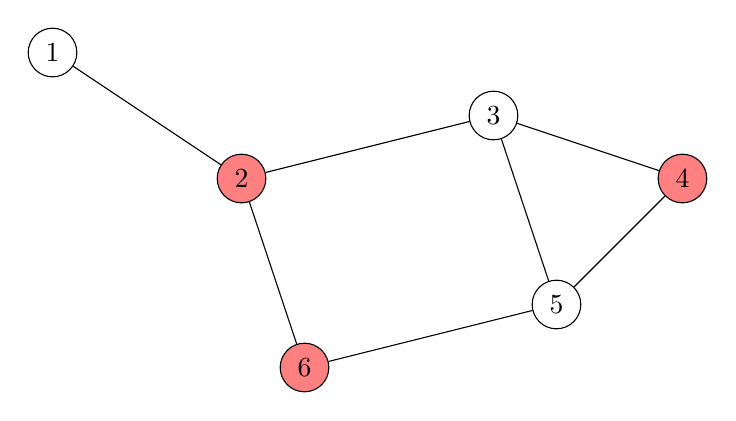
\begin{tikzpicture}
  			[scale=.8,auto=left,every node/.style={circle, draw,}]
  			\node (n6) at (1,10) {1};
  			\node (n5) at (8,9)  {3};
  			\node (n2) at (9,6)  {5};
  			\node [fill=red!50] (n3) at (5,5)  {6};
			\node [fill=red!50] (n4) at (4,8)  {2};
			\node [fill=red!50] (n1) at (11,8) {4};
		
  			\foreach \from/\to in {n6/n4,n4/n5,n5/n1,n1/n2,n2/n5,n2/n3,n3/n4}
    		\draw (\from) -- (\to);
		\end{tikzpicture}
	\end{center}
	\caption{A simple graph: terminal nodes are in red.}
    \label{graph}
\end{figure}

\begin{figure}[H]
	\begin{center}
		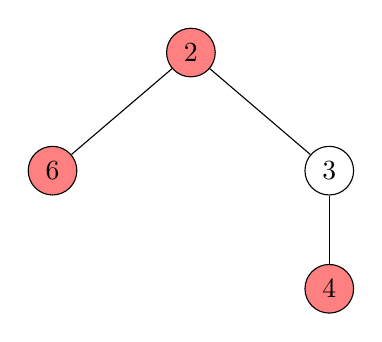
\begin{tikzpicture}[sibling distance=10em,
 			every node/.style = {shape= circle, draw, align=center,}]]
  			\node [fill=red!50] {2}
    		child { node [fill=red!50] {6} }
    		child { node {3}
      		child { node [fill=red!50] {4} }
			};
		\end{tikzpicture}
	\end{center}
	\caption{A possible Steiner Tree}
    \label{stree}
\end{figure}

A Steiner Tree for the graph is shown in Figure~\ref{stree}: $X$ is the set $\{2,3,4,6\}$. Note that, in general, there exist many possible STs for the same graph.

\subsection{Cut \& Count technique}
Before moving towards the algorithm for Steiner Tree, we need to give a slightly different definition of nice tree decomposition.
\theoremstyle{definition}
\begin{definition}
	A \emph{nice tree decomposition} is a tree decomposition $(X, T)$ where 
	$X = \{X_{t_1},...,X_{t_n}\}$, $T$ is a rooted tree, with empty root and leaves bags, and:
	\begin{itemize}
		\item every bag of $T$ has at most two children;
		\item if a bag $X_i$ has two children $X_j$ and $X_{j'}$, 
		then $X_i = X_j = X_j'$ (\emph{join node});
		\item if a bag $X_i$ has one children $X_j$, then either:
		\begin{itemize}
			\item $\mid X_i \mid = \mid X_j \mid + 1$ and $X_j \subset X_i$ 
			(\emph{introduce node})
			\item $\mid X_i \mid = \mid X_j \mid - 1$ and $X_i \subset X_j$ 
			(\emph{forget node})
		\end{itemize}
		\item if a bag $X_i$ is labelled with an edge $uv$ and has one child $X_j$ containing
		both $u$ and $v$, then $X_i = X_j$ (\emph{introduce edge node})
	\end{itemize}
	A bag of $T$ with no children is called a \emph{leaf}.
\end{definition}

A standard nice tree decomposition can be modified in polynomial time to meet the extra requirements given in the above definition. \\
Another important tool for the algorithm is the \emph{Isolation Lemma}:
\theoremstyle{definition}
\begin{definition}
	A function $\omega : U \rightarrow \mathbb{Z}$ \emph{isolates} a set family 
	$\mathcal{F} \subseteq 2^U$ if there is a unique $S' \in \mathcal{F}$ with
	$\omega(S') = min_{S \in \mathcal{S}} \omega(S)$, where, for $X \subseteq U$ we have
	$\omega(X) = \sum_{u \in X} \omega(u)$.
\end{definition}
\begin{lemma}
	Let $\mathcal{F} \subseteq 2^U$ be a set family over a universe $U$ with 
	$\mid \mathcal{F} \mid > 0$. For each $u \in U$, choose a weight 
	$\omega(u) \in \{1,2,...,N \}$ uniformly and independently at random. Then 
	$p[\omega \ isolates \ \mathcal{F}] \geq 1-\mid U \mid / N$.
\end{lemma}
Basically, the Isolation Lemma reduces a possibly large set of solutions to some problem to a unique one with a high probability, allowing for counting objects modulo 2. In this way, assuring that objects we are not interested in are counted an even number of times causes them to disappear. Since we deal with probability, the given algorithm is a randomized (MonteCarlo) algorithm which computes whether the set $\mathcal{S} \subseteq 2^U$ of solutions is empty or 
not. Cut\&Count consist then of two parts:
\begin{itemize}
	\item The \emph{Cut part}: consider the set $\mathcal{R}$ of possibly connected solutions,
	with $\mathcal{S} \subseteq \mathcal{R}$, thus relaxing the connectivity requirement and
	consider the set $\mathcal{C}$ of pairs $(X,C)$, with $X \in \mathcal{R}$ and $C$ being a
	consistent cut (i.e. a cut $(V_1,V_2)$ such that $u \in V_1$ and 
	$v \in V_2 \implies uv \not \in E$)
	\item The \emph{Count part}: compute $\mid \mathcal{C} \mid$ modulo 2. Since they are
	consistent with an even number of cuts, non-connected candidates 
	$X \in \mathcal{R} \setminus \mathcal{S}$ will disappear, leaving only connected candidates.
\end{itemize}
In the Count part we use the Isolation Lemma to get an odd number of solution. As a corollary, we obtain the following:
\begin{corollary}\label{cor}
	Let $\mathcal{S} \subseteq 2^U$ and $\mathcal{C \subseteq 2^{U \times (V \times V)}}$.
	Suppose that for every $W \in \mathbb{Z}$ we have:
	\begin{itemize}
		\item[1] $\mid \{ (X,C) \in \mathcal{C} \mid \omega(X) = W \} \mid \ \equiv \ 
		\mid \{ X \in \mathcal{S} \mid \omega(X) = W\} \mid$
		\item[2] $CountC(\omega,W,\mathcal{T}) \ \equiv \
		\mid \{ (X,C) \in \mathcal{C} \mid \omega(X) = W \} \mid$
	\end{itemize}
	Then the Cut\&Count algorithm returns \emph{no} if $\mathcal{S}$ is empty and \emph{yes}
	with probability at least $1/2$ otherwise.
\end{corollary}
\begin{algorithm}[H]
	\SetAlgoLined
	\SetKwInOut{Input}{Input}
	\SetKwInOut{Output}{Output}
	\Input{Set $U$; nice tree decomposition $\mathcal{T}$, procedure CountC
	accepting a $\omega : U \rightarrow \{ 1,...,N \}, W \in \mathbb{Z}$}
	\Output{Either \textbf{yes} if there exists a solution or \textbf{no} otherwise}
	\caption{The \textbf{Cut\&Count} procedure}
	\For{every $u \in U$} {
		Choose $\omega(u) \in \{ 1,...,2 \mid U \mid \}$ uniformly at random
	}
	\For{every $W$ s.t. $0 \leq W \leq 2 \mid U \mid^2$} {
		\If{CountC($\omega, W, \mathcal{T}$) $\equiv 1$} {
			\KwRet \textbf{yes}		
		}
	}
	\KwRet \textbf{no}
\end{algorithm}

\subsection{Applying Cut \& Count to Steiner Tree}
Now we can see how the above technique applies to Steiner Tree and how the resulting algorithm is parameterized via treewidth. \\
\begin{itemize}
	\item \textbf{\emph{Cut}} First we define the objects we are going to count.
	Given a wieght function $\omega : V \rightarrow \{ 1,...,N\}$, for any $W \in \mathbb{Z}$ let
	\[\mathcal{R}_W = \{ X \mid T \subseteq X \subseteq V, \omega(X) = W, \mid X \mid = k \}\]
	Also, define
	\[\mathcal{S}_W = \{ X \mid X \in \mathcal{R}_W, G[X] \ is \ connected \}\]
	The set $\bigcup_W \mathcal{S}_W$ is the set of solution: so the problem admits
	a solution if there is at least one $W$ such that $\mathcal{S}_W \not = \emptyset$. The set
	$\mathcal{R}_W$ contains the candidate (relaxed) solutions, where the only requirement left
	is that for each $X \in \mathcal{R}_W$ we have $T \subseteq X$. \\
	Let $u_1$ be a terminal: we define $\mathcal{C}_W$ as the set 
	$\{ (X, (X_1,X_2)) \}$ of consistently cut subgraphs such that $X \in \mathcal{R}_W$ and
	$u_1 \in X_1$.
	\item \textbf{\emph{Count}} The following lemma assures that the first condition of 
	corollary~\ref{cor} is actually met:
	\begin{lemma}
		Let $G,\omega,\mathcal{C}_W$ be as defined above. Then, for every $W$, we have
		$\mid \mathcal{S}_W \mid \equiv \mid \mathcal{C}_W \mid$.
	\end{lemma}
	The subprocedure \emph{CountC} is an application of dynamic programming, as stated by the following
	lemma:
	\begin{lemma}
		Given $G = (V,E)$, $T \subseteq V$, $k \in \mathbb{Z}$, $\omega : V \rightarrow \{ 1,...,N \}$ 
		and	a nice tree decomposition $\mathcal{T}$ of $G$, there exists an algorithm which computes 
		$\mid \mathcal{C}_W \mid \ mod \ 2$ for every $W$ such that $0 \leq W \leq kN$ in
		$3^t N^2 \mid V \mid^{O(1)}$.
	\end{lemma}
	We just give an intuition of how the subprocedure works. For cardinality $0 \leq i \leq k$ and weight
	$0 \leq w \leq kN$ we compute two sets. As a particular case, we have graphs with not
	weighted edges (each edge has weight $1$).
	\begin{itemize}
		\item $\mathcal{R}_x(i,w)$, containing the sets $X \subseteq V_x$ (for $V_x$ being the set of
		descendants of $x$) which can be extended to a candidate solution, having cardinality $i$ and
		weight $w$;
		\item $\mathcal{C}_x(i,w)$, containing consistently cut subgraphs respecting the given
		cardinality and weight.
	\end{itemize}
	Additionaly, we compute a number $\mathcal{A}_x(i,w,s)$, which counts those elements of $C_x(i,w)$
	which behave on vertices of the root as prescribed by a given sequence $s$. In simple terms,
	$s$ can be seen as a coloring and can be chosen among three values $\{ 0, 1_1, 1_2 \}$. \\
	Once the sets are defined, we can proceed to solve the subproblems on the nice tree decomposition
	of the graph in a bottom-up fashion. Then we have:
	\begin{itemize}
		\item \emph{\textbf{Leaf bag} x}: $\mathcal{A}_x(0,0,\emptyset) = 1$ and 
		$\mathcal{A}_x(i,w,s) = 0$ for all other choices of $i, w, s$.
		\item \emph{\textbf{Introduce vertex} v \textbf{bag} x}: we have three coloring to be considered
		for each vertex. Note that coloring a vertex as 0 means to exclude it from the solution, thus
		for $s = 0$ we must have $v \not \in T$. Recall also that, for an introduce vertex bag, we mean
		by $y$ the only child of $x$. Hence we obtain:
		\begin{itemize}
			\item $\mathcal{A}_x(i,w,s[v \rightarrow 0]) = [v \not \in T]\mathcal{A}_y(i,w,s)$
			\item $\mathcal{A}_x(i,w,s[v \rightarrow 1_1]) = \mathcal{A}_y(i-1,w-\omega(v),s)$
			\item $\mathcal{A}_x(i,w,s[v \rightarrow 1_2]) = 
			[v \not = v_1]\mathcal{A}_y(i-1,w-\omega(v),s)$
		\end{itemize}
		\item \emph{\textbf{Introduce edge} uv \textbf{bag} x}: here we must assure consistency between
		the endpoints of the edge. Thus we have:
		\begin{itemize}
			\item $\mathcal{A}_x(i,w,s) = [s(u) = 0 \vee s(v) = 0 \vee s(u) = s(v)]
			\mathcal{A}_y(i,w,s)$
		\end{itemize}
		\item \emph{\textbf{Forget vertex} v \textbf{bag} v}: in the child node, $v$ can have three
		colours. Then we must sum over all of them:
		\begin{itemize}
			\item $\mathcal{A}_x(i,w,s) = \sum_{\alpha \in \{0,1_1,1_2\}} \mathcal{A}_y(i,w,\alpha)$
		\end{itemize}
		\item \emph{\textbf{Join bag} x}: the only possibility to achieve the colouring $s$ is when
		both the children have the same colouring. Taking this into account, we sum up the contributions:
		\begin{itemize}
			\item $\mathcal{A}_x(i,w,s) = \sum_{i_1+i_2 = i + \mid s^{-1}(\{1_1,1_2\}) \mid} \\
			\sum_{w_1+w_2 = w + \omega(s^{-1}({1_1,1_2}))} \mathcal{A}_y(i_1,w_1,s)
			\mathcal{A}_z(i_2,w_2,s)$
		\end{itemize}
	\end{itemize}
	Combining dynamic programming with the given recursion we obtain the result stated in the lemma.
\end{itemize}
We can conclude by giving the following theorem.
\begin{theorem}
	There exists a MonteCarlo algorithm that given a tree decomposition of width $t$ solves Steiner Tree
	in running time $3^t \mid V \mid^{O(1)}$. This algorithm cannot give false positives and may give
	false negatives with probability at most $1/2$.
\end{theorem}

\section{More on applications of treewidth}
As said, several FPT algorithms for usually intractable problems can be obtained via treewidth:
\begin{itemize}
	\item if $G$ has "small" treewidth, using dynamic programming to compute an exact solution;
	\item if $G$ has "large" treewidth, using the structure of $G$ to compute an approximated
	solution.
\end{itemize}
Applications of treewidth involves many fields of computer science, as e.g. artificial intelligence, bioinformatics and networks. Consider, for instance, the aforementioned CSP variable elimination problem: here we want to decide whether an assignement of the variables on a given domain satisfies all the constraints. If a graph has treewidth $w$, then we can compute the solution in time $O(nd^{w+1})$, where $d$ is the maximum number of elements in the domain, by adopting a dynamic programming approach. \\
Another interesting application is the computation of the RNA folding problem. Here we want to compute an RNA folding with minimum free energy. This can be reduced to the problem of finding the maximum weighted independent set in the graph representing the set of the stacked nucleotide base pairs on an RNA sequence. Also this problem is FPT via treewidth.

\section{Conclusions}
The 5-approximation algorithm for treewidth represents mainly a theoretical result, due to the fact that the constant $c$ is large. Indeed, the $O(c^k nlogn)$ 3-approximation algortihm actually represents the best tradeoff. A further improvement for these results could be to provide an approximated algorithm for computing treewidth in $O(c^kn)$ where $c$ is a small constant. \\
Also finding an exact and efficient FPT-algorithm for treewidth is still an open problem: indeed, Bodlaender provided an exact time algorithm which runs in $O(k^{O(k^3)}n)$ time, hence applicable only on graphs of small width. Comsidering this, the 3-approximation algorithm on which the main algorithm is based, represents the best approximation for treewidth whose running time is single exponential in $k$ and polynomial in $n$. Also deciding if there are better approximation is still an open problem.

\newpage

\bibliographystyle{acm}
\bibliography{Report_FPT}

\end{document}